\subsection{Perceptrón}
Un perceptrón es un tipo de neurona artificial que toma varias entradas binarias, $x_1 , x_2 , . . .,$ y produce una única salida binaria:
\begin{equation}
    \text{salida}=\begin{cases}
    0~~\text{si}~~\sum w_ix_i\leq \text{umbral}\\
    1~~\text{si}~~\sum w_ix_i\geq\text{umbral}
    \end{cases}
\end{equation}

donde se introducen los pesos, $w_1, w_2 , ...$ números reales que expresan la importancia de las respectivas entradas para la salida. La salida de la neurona ($0$ o $1$), se determina en función de si la suma ponderada $\sum_j w_j x_j$ es menor o mayor que un valor umbral. Al igual que las ponderaciones, el umbral es un número real que constituye un parámetro de la neurona. 

La representación gráfica de un perceptrón es 
\begin{figure}[h!]
    \centering
    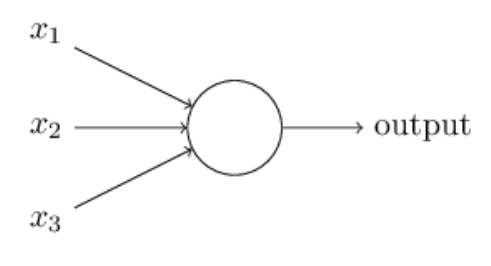
\includegraphics[width=0.25\linewidth]{imagen.png}
\end{figure}



Simplificando la descripción de los perceptrones. La condición $
\sum_j w_j x_j > \text{umbral}$ es compleja, y podemos hacer dos cambios de notación para simplificarla. El primer cambio consiste en escribir $\sum_j w_jx_j$ como un producto escalar, $w \cdot x = \sum_j w_j x_j$ , donde $w$ y $x$ son vectores cuyos componentes son los pesos y las entradas, respectivamente. El segundo cambio consiste en desplazar el umbral al otro lado de la desigualdad y reemplazarlo por lo que se conoce como el sesgo (bias) del perceptrón, $b = - \text{umbral}$. Utilizando el sesgo en lugar del umbral, la regla del perceptrón se puede reescribir:

\begin{equation}
    \text{salida}=\begin{cases}
    0~~\text{si}~~w\cdot x +b\leq 0\\
    1~~\text{si}~~w\cdot x+b\geq 0
    \end{cases}
\end{equation}




Los perceptrones se pueden usar para calcular las funciones lógicas elementales que solemos considerar como computación subyacente, como AND, OR y NAND. Por ejemplo, supongamos que tenemos un perceptrón con dos entradas, cada una con un peso de $-2$ y un sesgo general de $3$, entonces vemos que la entrada $00$ produce la salida 1, ya que $(-2)\times 0 + (-2)\times 0 + 3 = 3$ es positivo. Cálculos similares muestran que las entradas 01 y 10 producen la salida 1. Pero la entrada 11 produce la salida 0, ya que $(-2)\times 1 + (-2)\times 1 + 3 = -1$ es negativo. Por lo tanto, nuestro perceptrón implementa una puerta NAND.

\section{Modelos de redes}

\subsection{Reed feedfoward}

Una red de propagación hacia adelante (también conocida como red neuronal feedforward) es un tipo de red neuronal artificial donde la información fluye solo en una dirección, desde las capas de entrada a las capas de salida, sin conexiones cíclicas. Tomando como ejemplo.
\begin{figure}[h!]
    \centering
    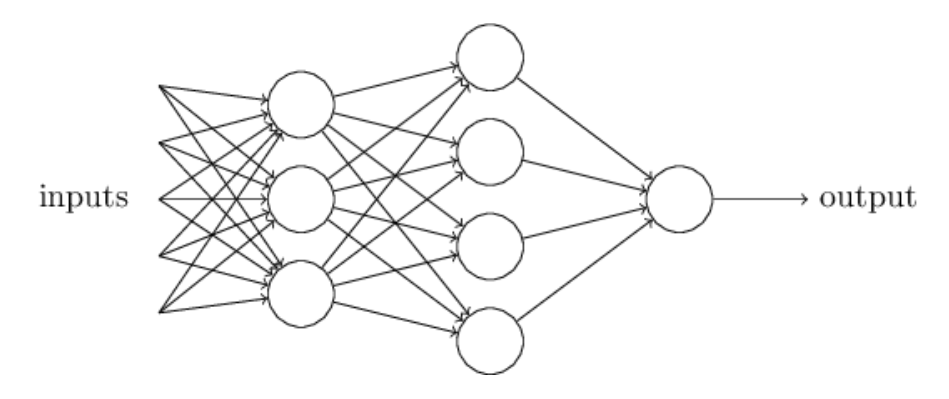
\includegraphics[width=0.5\linewidth]{imagen2.png}
\end{figure}
Lo que llamaremos la primera capa de perceptrones, toma tres decisiones muy simples, sopesando la evidencia de entrada. ¿Qué pasa con los perceptrones de la segunda capa? Cada uno de estos perceptrones toma una decisión sopesando los resultados de la primera capa de toma de decisiones. De esta manera, un perceptrón de la segunda capa puede tomar una decisión a un nivel más complejo y abstracto que los perceptrones de la primera capa. Y el perceptrón de la tercera capa puede tomar decisiones aún más complejas. De esta manera, una red de perceptrones de múltiples capas puede participar en una toma de decisiones sofisticada.

El ejemplo de NAND muestra que podemos usar perceptrones para calcular funciones lógicas simples. De hecho, podemos usar redes de perceptrones para calcular cualquier función lógica. Esto se debe a que la puerta NAND es universal para la computación; es decir, podemos construir cualquier computación a partir de puertas NAND.

\subsection{Redes recurrentes}

Las redes neuronales recurrentes (RNNs, por sus siglas en inglés) son un tipo de red neuronal profunda que se diseñaron para procesar datos secuenciales, es decir, datos que tienen un orden o secuencia. A diferencia de las redes neuronales tradicionales (que procesan datos de forma independiente en cada capa), las RNNs tienen una estructura que permite que la información persista a través del tiempo, lo que les permite recordar información pasada y usarla para predecir o clasificar información futura.

\subsubsection{Red de Hopfield}

Una red de Hopfield es un tipo de red neuronal recurrente que se utiliza para el almacenamiento y recuperación de patrones, funcionando como una forma de memoria asociativa. Fue propuesta por John Hopfield en 1982.

La red de Hopfield es formalmente análoga al modelo de Ising de la física estadística. En el modelo de Ising. Los "espines" $s_i$ pueden estar en estado $+1$ o $-1$. Hay interacciones entre espines vecinas, caracterizadas por acoplamientos $J_{ij}$.

En la red de Hopfield, los pesos $w_{ij}$ juegan un papel similar a los acoplamientos $J_{ij}$, y el estado de la red corresponde a una configuración de espines. La analogía es tan directa que se puede definir una función de energía donde $\theta_i$ es el umbral (bias) de activación de la neurona $i$.

\begin{equation}
E(\mathbf{s}) = -\frac{1}{2} \sum_{i,j=1}^{N} w_{ij} s_i s_j + \sum_{i=1}^{N} \theta_i s_i
\end{equation}

La red de Hopfield funciona como un sistema de \textbf{memoria asociativa}, capaz de recuperar patrones completos a partir de versiones incompletas o ruidosas. La decisión que toma la red corresponde al patrón almacenado más cercano (en términos de similitud) al estado inicial que se le proporciona.

En el estado inicial se proporciona un patrón de entrada $\mathbf{s}^{(0)}$ que puede estar incompleto o contaminado por ruido cada neurona $i$ calcula su entrada neta \[
    h_i = \sum_{j=1}^{N} w_{ij} s_j - \theta_i
    \] y actualiza su estado mediante la regla: \[
    s_i(t+1) = \text{sgn}(h_i)
    \] La actualización puede realizarse: Tras varias actualizaciones, el sistema alcanza un estado estable (mínimo de energía). Ese estado final es la ``decisión'' de la red: el patrón memorizado que mejor coincide con la entrada inicial.

Existen diversas reglas de aprendizaje que pueden utilizarse para almacenar información en la memoria de la red de Hopfield. Es deseable que una regla de aprendizaje tenga las dos propiedades siguientes
\begin{itemize}
    \item Local : una regla de aprendizaje es local si cada peso se actualiza utilizando la información disponible para las neuronas en cada lado de la conexión asociada con ese peso en particular.

    \item Incremental : Se pueden aprender nuevos patrones sin usar información de los patrones antiguos que también se usaron para el entrenamiento. Es decir, cuando se usa un nuevo patrón para el entrenamiento, los nuevos valores de los pesos dependen únicamente de los valores antiguos y del nuevo patrón. 

\end{itemize}
